\documentclass[english,12pt,a4paper]{report}
\usepackage[T1]{fontenc}
\usepackage[top=3cm, bottom=3cm]{geometry}
\usepackage{graphicx}
\usepackage{mathtools}
\usepackage{amssymb}
\usepackage{amsthm}
\usepackage{thmtools}
\usepackage{xcolor}
\usepackage{nameref}
\usepackage{babel}
\usepackage{url}
\geometry{
	a4paper,
	total={170mm,257mm},
	left=25mm,
	right=25mm,
	top=27mm,
}
\usepackage{subcaption}
\usepackage{babel}
\newcommand*{\captionsource}[2]{%
	\caption[{#1}]{%
		#1%
		\\\hspace{\linewidth}%
		\textbf{Source:} #2%
	}%
}
\usepackage{physics}
\usepackage[export]{adjustbox}
\usepackage{caption}
\usepackage{amsmath,cite,times,enumerate,enumitem,amsfonts,amssymb,pdfpages,makeidx,graphicx,array, multirow}
\usepackage[most]{tcolorbox}
\usepackage{hyperref}
\hypersetup{colorlinks=true, linkcolor=blue,citecolor=red,urlcolor=cyan}
\title{Quantum Machine Learning}
\author{Ashis Nayak}
\begin{document}
	\begin{titlepage}
		\begin{center}
			\vspace{3em}
			{\LARGE \text{} \\ \textbf{Quantum Approximate Optimization Algorithm and The Ising Model }}\\
			\vspace{1em}
			{\large \text{Reading Project (sem 6)}\\
				\text{Final Report}\\
				\vspace{2em}
				\textit{submitted by}\\\textbf{Ashis Nayak}\\\text{School of Physical Sciences}\\\text{
					UM-DAE-CEBS, Mumbai}}
			\vspace{2em}
			\begin{figure}[!htb]
				\centering
				
\includegraphics[height=0.21\textheight]{logo 2}
			\end{figure}
			\\
			{\large \vspace{2em}
				\textit{Under the Guidance of}\\\textbf{Prof. Anuradha Mishra}\\\text{School of Physical Sciences}\\\text{
					UM-DAE-CEBS, Mumbai}\\
				\vspace{1em}
				\text{Date:{12/05/2026}}}
		\end{center}
	\end{titlepage}
	\pagenumbering{roman}
	\section*{\huge Acknowledgement}
		\addcontentsline{toc}{section}{Acknowledgement}
{\large I would like to express my sincere gratitude to Dr. Anuradha Mishra, UM DAE Centre for Excellence in Basic Sciences, for her guidance and support throughout this semester for the reading project. Her guidance and encouragement at every stage were invaluable and helped me achieve my goal of understanding and delving deep into this topic.

I am especially thankful for her patience in addressing my questions and for continuously motivating me to think critically and explore concepts more deeply. This project has been a highly enriching experience, and I am grateful for the opportunity to work under her supervision. I also extend my thanks to my peers and seniors who were always present to answer my questions , discuss and rectify my doubts. I would like to thank my senior A.R Bathri Narayan and my peer U Manasvi Maiya and the students of University of Mumbai who were present for my presentations and discussions which added a lot of value and input that went into this report.
}
	\newpage
	\section*{\centering  \LARGE Abstract}
	\addcontentsline{toc}{section}{Abstract}
	This report presents a conceptual introduction to the Quantum Approximate Optimization Algorithm (QAOA) through its connection to machine learning, the Ising model, and combinatorial optimization. The discussion begins with a brief overview of machine learning, including common learning tasks, basic data representations, similarity measures, and the role of loss functions and generalization. These ideas provide the background for viewing optimization problems in a mathematical framework that is shared by both classical and quantum methods.
	
	The report then introduces the Ising model as a fundamental model of interacting spins and explains how its groundstate search can be interpreted as an optimization problem. The mapping between the Ising formulation and quadratic unconstrained binary optimization (QUBO) is described, followed by a discussion of quantum time evolution, transverse fields, adiabatic quantum computing, and quantum annealing. This motivates the transition to variational quantum algorithms, with particular emphasis on how QAOA can be understood as a discretized approximation to adiabatic evolution using alternating applications of cost and mixing Hamiltonians.
	
	Finally, the Max-Cut problem is used as a concrete example to illustrate how a graph optimization problem can be encoded into the QAOA framework. The report shows how the objective function is translated into a cost operator, how the corresponding unitary operations are constructed, and why this problem serves as a natural benchmark for quantum optimization. A QISKIT implementation of the same is presented in the final section showing a simulation of this problem with expected outcomes.
	Overall, the report aims to build an intuitive and mathematical understanding of how QAOA emerges from physical models and how it can be applied to practically relevant optimization problems.
	
	\tableofcontents
	\newpage
	\chapter{Introduction To Machine Learning}
	\section{Machine Learning}
	Machine learning is a branch of artificial intelligence concerned with developing algorithms that learn patterns from data and use those patterns to make predictions, classifications, or decisions without being explicitly programmed for every individual task. Instead of following only fixed rules, a machine learning model improves its performance by identifying structure in past observations and applying that knowledge to new inputs.\pagenumbering{arabic} 
	
	\section{Types of Machine Learning Algorithms}
	Machine learning algorithms can be organized according to the kind of task they solve. Some algorithms predict a continuous numerical quantity, some assign an input to one of a few discrete categories, and others try to discover structure in unlabeled data. In this section, we briefly discuss a few foundational problems and the methods commonly used to address them. \cite{Djordjevic2021}
	
	\subsection{Linear Regression}
     Linear regression is a supervised learning algorithm used to model the relationship between input variables and a continuous output variable. The model assumes that the prediction can be written as a linear combination of the input features.
	
	Suppose the input is represented by $x=(x_1,x_2,\dots,x_n)$. Then a linear regression model predicts the target value as
	\begin{equation}
		\hat{y} = w_1x_1 + w_2x_2 + \cdots + w_nx_n + b,
	\end{equation}
	where $w_i$ are the model parameters and $b$ is the bias term.
	

	\begin{itemize}
		\item It is mainly used when the target variable is continuous, such as temperature, stock value, or house price.
		\item Training usually involves minimizing the mean squared error between the predicted values and the true values.
		\item The learned coefficients provide an interpretable measure of how each feature influences the output.
		\item Although simple, linear regression often serves as a baseline model for more complicated regression tasks.
	\end{itemize}
	
	\subsection{Binary Classification}
	Binary classification is a supervised learning problem in which each data point must be assigned to one of two possible classes. Typical examples include spam or not spam, diseased or healthy, and accepted or rejected.
	

	\begin{itemize}
		\item The output is discrete, usually encoded as $0$ and $1$.
		\item Binary classification differs from regression because the goal is not to predict a continuous value but to assign a label.
		\item Performance is commonly evaluated using accuracy, precision, recall, F1-score, and the ROC curve.
		\item Many algorithms can solve binary classification problems, including logistic regression, support vector machines, decision trees, and neural networks.
	\end{itemize}
	
	\subsection{Clustering Problem}
	Clustering is an unsupervised learning problem in which the aim is to divide a dataset into groups, called clusters, such that points within the same cluster are more similar to each other than to points in other clusters.
	
	Unlike supervised learning, clustering does not require labeled examples. Instead, the algorithm tries to infer the hidden structure of the data directly from the features. One of the most widely used methods is K-means clustering, which partitions the data into $K$ clusters by iteratively updating cluster centers and assigning points to the nearest center.
	
	\begin{itemize}
		\item Clustering is useful for exploratory data analysis, pattern discovery, image segmentation, and customer grouping.
		\item The number of clusters may be chosen in advance or estimated using heuristic methods such as the elbow method or silhouette score.
		\item Since there are no ground-truth labels, evaluating clustering quality is generally more difficult than evaluating supervised tasks.
		\item Common clustering algorithms include K-means, hierarchical clustering, and grover based K-means.
	\end{itemize}
	
	\subsection{Principal Component Analysis (PCA)}
	Principal Component Analysis is an unsupervised dimensionality reduction technique used to transform a dataset with many correlated variables into a new set of orthogonal variables called principal components.
	
	The first principal component is the direction along which the data has the largest variance. The second principal component is orthogonal to the first and captures the next largest variance, and so on. By keeping only the first few components, one can represent the data in a lower-dimensional space while preserving most of its important variation.

	\begin{itemize}
		\item PCA is often used for visualization, noise reduction, feature extraction, and data compression.
		\item It is especially useful when the original features are highly correlated.
		\item The principal components are obtained from the eigenvectors of the covariance matrix, or equivalently from singular value decomposition.
		\item PCA is not itself a classifier or regressor; rather, it is a preprocessing tool that can improve the performance of other learning algorithms.
	\end{itemize}
	\begin{figure}[!htb]
		\centering
		\tcbox[colback=white, boxsep=0em]{
		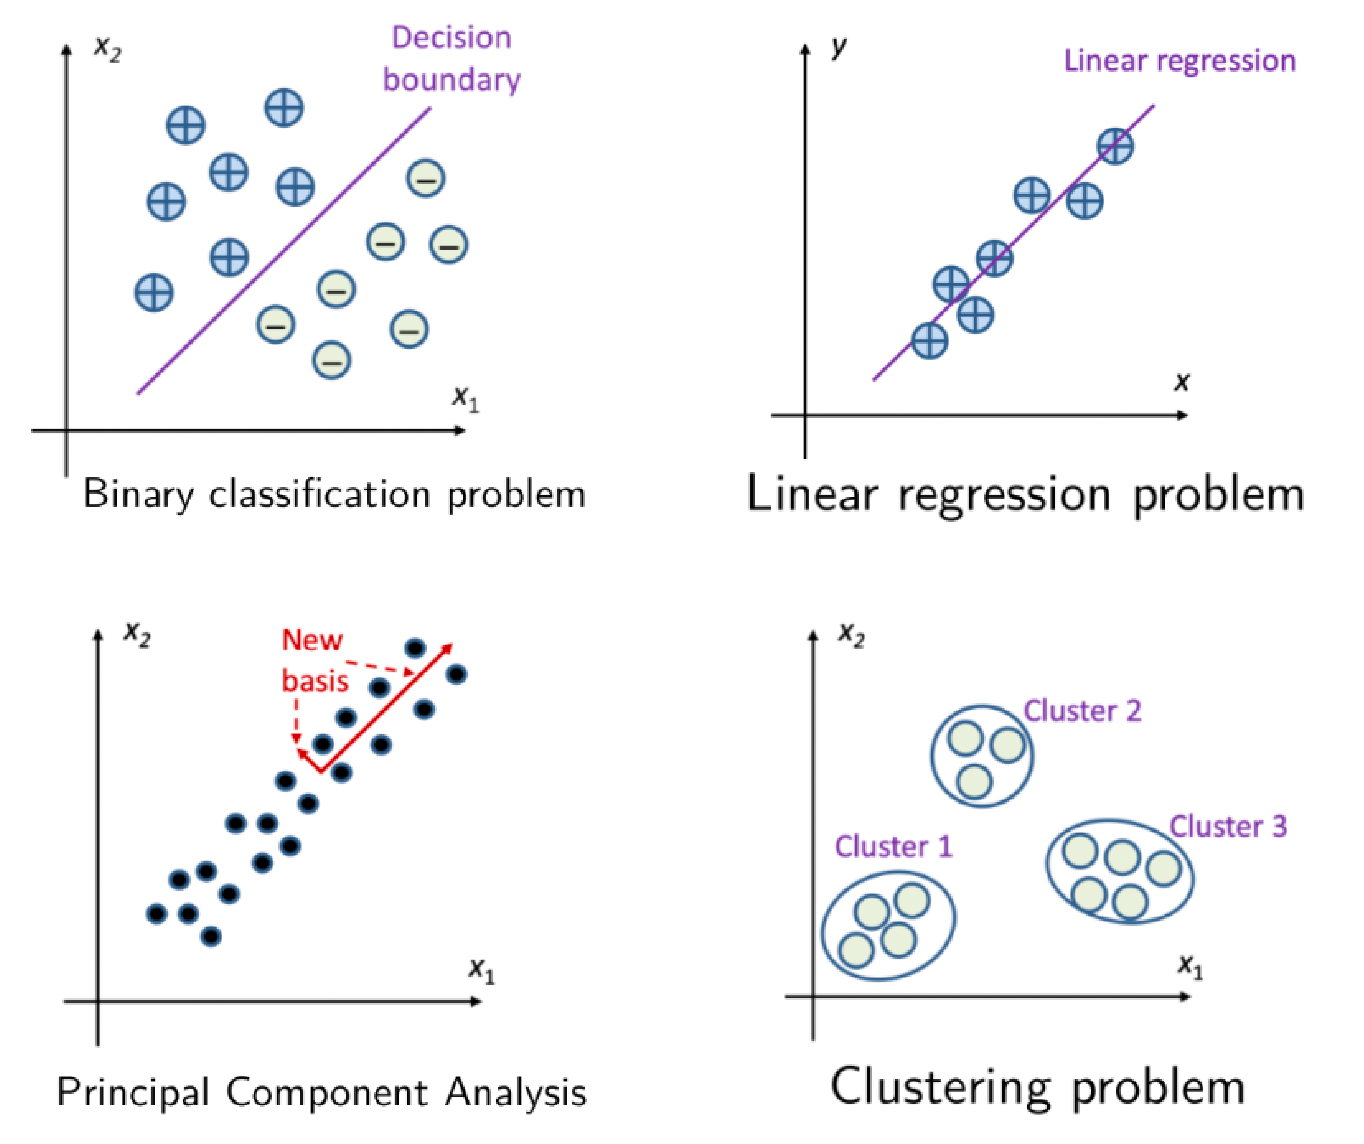
\includegraphics[width=0.9\linewidth]{img1}}
		\caption{Different type of data set and the techniques used for applying Machine Learning on them \cite{Djordjevic2021}.}
		\label{fig:img1}
	\end{figure}
	\newpage
\section{Important Terminologies}
The following are some important terminologies used in Machine Learning and their definitions \cite{Djordjevic2021}:
\subsection{Feature Vector}
A feature vector is the mathematical representation of a data point in terms of its measured attributes. If a dataset has $d$ features, then each sample can be represented as a vector in a $d$-dimensional space:
\[
x_j=\sum_{i=1}^{d}x_{ij}e_i=
\begin{bmatrix}
	x_{1j}\\x_{2j}\\\vdots\\x_{dj}
\end{bmatrix},
\]
where the basis vector $e_i$ corresponds to the $i$th feature and $j$ labels the data instance. This representation is central in machine learning because most learning algorithms operate on vectors of this form. Once the data are written as feature vectors, one can compare samples, compute distances, and define predictive models in a systematic way.

\subsection{Cosine Similarity}
The cosine similarity between two vectors is
\[
\cos(x_j,x_k)=\frac{x_j^Tx_k}{\norm{x_j}\,\norm{x_k}}.
\]
It measures the alignment between two vectors and is useful when direction is more important than magnitude. A cosine similarity close to $1$ indicates that two samples point in nearly the same direction and are therefore similar in pattern, whereas a value close to $0$ indicates weak similarity. This measure is commonly used in text analysis, information retrieval, and high-dimensional datasets where the overall scale of the vector is less important than the relative composition of features.

\subsection{Hamming Distance}
For binary-valued data, the Hamming distance is defined as
\[
d_H(x_j,x_k)=\sum_{i=1}^{d}x_{ij}\oplus x_{ik}.
\]
It counts the number of positions at which two binary strings differ. Therefore, it is a natural measure of dissimilarity for bit strings, binary codes, and discrete spin-like variables. In problems involving binary data, the Hamming distance provides a simple way to quantify how many feature values must change in order to transform one configuration into another.

\section{Loss Functions and Generalization}
The loss function $L(y,f(x))$ measures the discrepancy between the true output $y$ and the predicted output $f(x)$. It is one of the key ingredients of machine learning because it tells us how well a model performs on individual examples. During training, model parameters are adjusted so as to reduce the overall loss over the dataset.

\subsection{Common Loss Functions}
Two standard choices for regression are:
\begin{itemize}
	\item \textbf{Squared error:} \[L(y_j,f(x_j))=[y_j-f(x_j)]^2\]
	This loss penalizes large errors more strongly because the deviation is squared, which makes it especially useful when large mistakes should be discouraged.
	\item \textbf{Absolute error:} \[L(y_j,f(x_j))=\abs{y_j-f(x_j)}\]
	This loss grows linearly with the prediction error and is often more robust to outliers than squared error.
\end{itemize}
These loss functions are widely used in regression problems where the target variable is continuous.

\subsection{Empirical Risk}
The average loss on the training dataset is called the empirical risk or training error:
\[
E=\frac{1}{n}\sum_{j=1}^{n}L(y_j,f(x_j)).
\]
It summarizes how well the model fits the observed training samples. Minimizing the empirical risk is the basic objective in many machine learning methods. However, a model that achieves a very small training error is not necessarily useful if it simply memorizes the training data.

\subsection{Generalization Error}
The generalization error measures performance on previously unseen data drawn from the underlying distribution:
\[
E_{GE}=\int_{x\in X,\,y\in Y}L(y,f(x))p(y,x)\,dx\,dy.
\]
This quantity is more important than the training error because the real aim of machine learning is to perform well on new examples rather than only on the data used for training. In practice, since $p(y,x)$ is usually unknown, generalization is estimated using validation or test data. A good model should achieve low training error and also generalize well, thereby avoiding both underfitting and overfitting.

\chapter{The Ising Model}
\section{Introduction to the Ising Model}
The Ising model is one of the simplest and most important models in statistical physics for studying collective behavior in systems of interacting magnetic moments. It was originally introduced to understand ferromagnetism, that is, the tendency of microscopic magnetic dipoles inside a material to align in a common direction. Despite its simple mathematical structure, the model captures essential physical ideas such as ordering, thermal disorder, and phase transitions, and for this reason it has become a standard framework in both physics and optimization theory.

In the Ising model, each spin variable takes one of two possible values, $\sigma_i\in\{-1,1\}$, which may be interpreted as an ``up'' spin or a ``down'' spin. These spins are placed on the vertices of a graph, most commonly on a one-dimensional chain or a two-dimensional lattice, and each spin interacts primarily with its nearest neighbors. The system may also be influenced by an external magnetic field, which tends to bias the spins toward a preferred orientation. When neighboring spins align, the interaction energy is lowered, so the system energetically favors ordered configurations. On the other hand, thermal fluctuations arising from finite temperature tend to randomize the spin orientations and disrupt this order. The balance between these competing effects, interaction driven ordering and temperature driven disorder determines the macroscopic behavior of the material. As temperature or external parameters are varied, the model can exhibit phase transitions, where the qualitative behavior of the system changes abruptly, for example from a magnetized ordered phase to a disordered paramagnetic phase.
	
\section{Hamiltonian Formulation}
The Hamiltonian of the Ising model is
\[
H(\sigma)=-\sum_{\langle i,j \rangle}J_{ij}\sigma_i\sigma_j-\mu \sum_i h_i\sigma_i.
\]
Here, $J_{ij}$ denotes the interaction strength between the $i$th and $j$th sites, $h_i$ denotes the strength of the external magnetic field acting on the $i$th spin site, $\mu$ is the magnetic moment, and $\langle i,j \rangle$ denotes nearest-neighbor pairs.

The sign of $J_{ij}$ determines the type of interaction:
\begin{itemize}
	\item $J_{ij}>0$: ferromagnetic interaction,
	\item $J_{ij}<0$: antiferromagnetic interaction,
	\item $J_{ij}=0$: no interaction.
\end{itemize}
If $h_i>0$, the $i$th spin tends to align with the external field in the positive direction.

\section{Boltzmann Distribution and Optimal Configuration}
The probability of a configuration is described by the Boltzmann distribution:
\[
P_\beta(\sigma)=\frac{1}{Z_\beta}e^{-\beta H(\sigma)}, \qquad \beta=\frac{1}{k_B T},
\]
where $\beta$ is the inverse temperature and $Z_\beta$ is the partition function,
\[
Z_\beta = \sum_{\sigma}e^{-\beta H(\sigma)}.
\]
If the interaction matrix is denoted by $J=(J_{ij})$, then the optimum configuration may be written as
\[
\hat{\sigma}=\arg\min_{\sigma}(\sigma^T J\sigma + h^T\sigma).
\]
This optimization viewpoint is important because it connects the Ising model to classical and quantum optimization problems. Thus it is natural to map this problem to a known optimization problem called the \emph{\textbf{QUBO problem}}.
	
\section{QUBO Formulation}\label{QUBO}
Quadratic unconstrained binary optimization (QUBO) is a standard way of expressing optimization problems using binary decision variables. In this framework, each variable can take only the value $0$ or $1$, and the aim is to find the binary string that minimizes a quadratic cost function. The term \emph{quadratic} means that the objective includes both individual variable contributions and pairwise interaction terms, while \emph{unconstrained} means that any conditions from the original problem are typically absorbed into the objective function through penalty terms. For this reason, many combinatorial optimization problems can be rewritten in QUBO form. 

In a QUBO problem, the variables are binary, $x_i\in \{0,1\}$, and the objective function is quadratic:
\[
\hat{x}=\arg\min_x(x^T W x + b^T x).
\]
The Ising problem can be reformulated as a QUBO problem by defining $\sigma_i=2x_i-1$, taking $\mu=1$, and identifying $b_i=h_i$ as the bias term.

The Ising Hamiltonian can also be written in terms of Pauli operators as
\[
\hat{H}=-\sum_{\langle i,j \rangle}J_{ij}\sigma_i^{Z}\sigma_j^{Z} -\sum_i h_i\sigma_i^Z,
\]
where
\[
\sigma^Z = Z =
\begin{bmatrix}
	1&0\\
	0&-1
\end{bmatrix}.
\]
	\section{Time Evolution and Transverse Field}
	The quantum state evolves according to
	\[
	i\hbar\frac{dU}{dt}=HU.
	\]
	For a time-independent Hamiltonian,
	\[
	U=e^{-iHt/\hbar}.
	\]
	
	With a transverse field, the Hamiltonian becomes
	\[
	\hat{H}=-\sum_{\langle i,j\rangle}J_{ij}\sigma_i^Z\sigma_j^Z-\sum_i h_i\sigma_i^X,
	\]
	where
	\[
	\sigma^X=
	\begin{bmatrix}
		0&1\\
		1&0
	\end{bmatrix}.
	\]
	The transverse field introduces quantum fluctuations that allow transitions between spin configurations.
	\\
	The discussion so far has established how the Ising model can be expressed in both classical and quantum language, and how its ground-state search can be interpreted as an optimization problem. This naturally leads to the next question: how can one use quantum dynamics to reach or approximate this ground state efficiently? An approximate solution is provided by adiabatic quantum computing and quantum annealing.
	
	\chapter{Adiabatic Quantum Computing and Quantum Annealing}
	\section{Adiabatic Principle}
	An adiabatic process is a process that changes slowly enough that the system can continuously adapt its configuration. If the system starts in the ground state of an initial Hamiltonian $H_0$, then under sufficiently slow evolution it will remain close to the instantaneous ground state and eventually end in the ground state of the final Hamiltonian $H_1$. This statement is the content of the adiabatic theorem, originally formulated by Born and Fock.
	
	The time dependent Hamiltonian for this process is in general written as:
	\begin{equation}
		H(t)= (1-t)H_0 + tH_1, \qquad t\in[0,1].
	\end{equation}
	As the parameter $t$ increases from $0$ to $1$, the system moves from the initial Hamiltonian $H_0$ to the target Hamiltonian $H_1$, provided the evolution is sufficiently slow and the ground state remains non-degenerate.
	
	\section{Adiabatic Evolution for the Ising Model}
	For the Ising model, one typically chooses the initial Hamiltonian to be
	\[
	H_0=-\sum_i X_i,
	\]
	which describes the interaction of a transverse field with the spin sites. The final Hamiltonian is chosen as
	\[
	H_1 = -\sum_{\langle i,j \rangle}J_{ij}Z_iZ_j - \sum_i h_iX_i.
	\]
	The system is then guided from an easily prepared initial ground state toward the ground state of the problem Hamiltonian. This idea forms the basis of quantum annealing. 
	\begin{figure}[!htb]
		\centering
		\tcbox[boxsep=0em,colback=white]{
		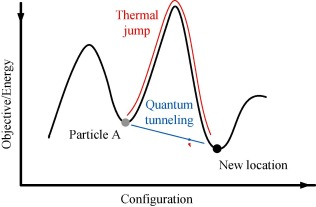
\includegraphics[width=0.7\linewidth]{qann}}
		\caption{Quantum annealing \cite{Djordjevic2021}.}
		\label{fig:qann}
	\end{figure}
	\\\\\\\\\\\\\\\\
	The beauty of Quantum Annealing lies in the fact that quantum mechanically wavefunctions can tunnel through barriers unlike classical particles. Thus approaching a global minimum becomes easier and requires lower energy than thermal excitation or any other classical way. Quantum computers that are specifically designed to carry out such annealing tasks are called \textbf{\emph{Quantum Annealers}}.  
	
	\chapter{Variational Quantum Algorithms and Quantum Approximate Optimization Algorithm}
	\section{VQE}
	Quantum circuits are inherently prone to noise and operational errors, which makes deep gate-based implementations difficult on near-term quantum hardware. This motivates the use of variational quantum circuits, which combine quantum state preparation with classical optimization. Such methods are particularly suitable for noisy and imperfect quantum computers.
	
	One important example is the variational quantum eigensolver (VQE), which estimates the ground-state energy of a Hamiltonian by preparing a parameterized quantum state and minimizing the expectation value of the Hamiltonian with respect to the circuit parameters.
	
	\begin{figure}[htbp]
		\centering
		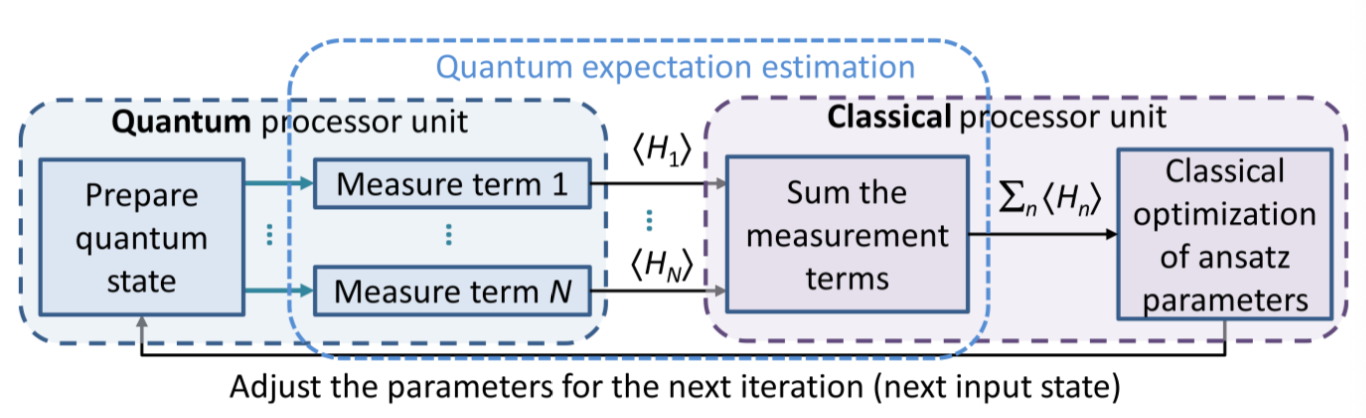
\includegraphics[width=0.8\linewidth]{qac1}
		\caption{Variational quantum eigensolver \cite{Djordjevic2021}.}
		\label{fig:qac1}
	\end{figure}
	
	\section{QAOA}
	The key idea behind the Quantum Approximate Optimization Algorithm (QAOA) is to approximate the adiabatic evolution pathway by a sequence of discrete unitary operations. Let $U(t)$ denote the ideal continuous evolution operator. The final operator $U(T)$ can be approximated by a product of simpler operators if the Hamiltonian changes gradually enough.
	
	A discretized step may be written as \cite{Djordjevic2021}
	\begin{equation}
		U'_k = e^{-i\frac{T}{p}H(kT/p)} = e^{-i\frac{T}{p}(\frac{k}{p}H_f +(1-\frac{k}{p})H_0)}.
	\end{equation}
	Here, the total computation time $T$ is divided into $p$ intervals.
	
	Using the Campbell--Baker--Hausdorff theorem, one may approximate this by a product of separate evolutions under $H_f$ and $H_0$:
	\begin{equation}
		U'_k \cong U(H_f,\tfrac{k}{p}\tfrac{T}{p}) U(H_0,(1-\tfrac{k}{p})\tfrac{T}{p}).
	\end{equation}
	More generally, the $k$th step can be written as
	\begin{equation}
		U'_k = U(H_f,\gamma_k ) U(H_0, \beta_k), \qquad \beta_k +\gamma_k = \triangle T_k, \qquad \sum_{k=1}^{p} \triangle T_k=T.
	\end{equation}
	This decomposition need not be uniform, which gives flexibility in optimizing the parameters.
	
	\section{Trotterized Approximation}\label{trot}
	Thus, one alternates the evolution under $H_0$ and $H_f$ to approximate the adiabatic pathway:
	\begin{equation}
		U(T)\cong U(H_f,\gamma_p)U(H_0,\beta_p)\dots U(H_f,\gamma_1)U(H_0,\beta_1).
	\end{equation}
	This approximation is commonly known as Trotterization or the Trotter--Suzuki decomposition.
	
	\begin{figure}[!htb]
		\centering
		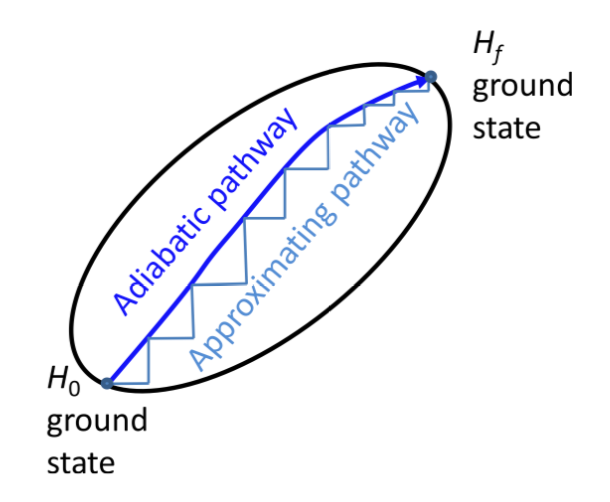
\includegraphics[width=0.55\linewidth]{qac}
		\caption{Approximation of the adiabatic pathway \cite{Djordjevic2021}.}
		\label{fig:qac}
	\end{figure}

	Because the chosen initial Hamiltonian is $H_0=-\sum_i X_i$, its ground state is the tensor product of $\ket{+}=\frac{\ket{0}+\ket{1}}{\sqrt{2}}$ over all qubits:
	\begin{equation}
		\ket{\psi_0}=\ket{+}^{\otimes N}=\frac{1}{\sqrt{2^N}}\sum_z \ket{z}, \qquad z\in \{0,1\}^N.
	\end{equation}
	The final state after $p$ QAOA steps is then
	\begin{equation}\label{eq:evol}
		\ket{\psi_f (\beta,\gamma)}=\ket{\beta,\gamma}=U(H_f,\gamma_p)U(H_0,\beta_p)\dots U(H_f,\gamma_1)U(H_0,\beta_1)\ket{\psi_0}.
		\end{equation}
		
		Suppose the optimization objective is
		\begin{equation}
		C_{\max}=\max_{z}{C(z)} = \max_{z}{\sum_{k=1}^{m}C_k(z)}, \qquad z\in \{0,1\}^N,
		\end{equation}
		where each $C_k$ encodes a Boolean or weighted constraint.
		
		\section{Cost Operator and Expectation Value}
		The objective function can be represented by an operator $C$ satisfying
		\begin{equation}
		C\ket{z}=\sum_{k=1}^{m}C_k (z) \ket{z} = f(z) \ket{z}.
		\end{equation}
		The eigenvalues of $C$ are therefore the values $f(z)=\sum_k C_k(z)$, and the largest eigenvalue is $C_{\max}=f(z_{\max})$.
	
	For an arbitrary state $\ket{\psi}=\sum_z \alpha_z\ket{z}$, the expectation value of the cost operator is bounded by the maximum value of the objective function:
	\begin{equation}
		\bra{\psi}C\ket{\psi}\leq f(z_{\max}).
	\end{equation}
	For the initial equal superposition state, one obtains
	\begin{equation}
		\bra{\psi_0}C\ket{\psi_0} = \frac{1}{2^N}\sum_{z\in \{0,1\}^N} f(z).
	\end{equation}
	The probability of obtaining the maximizing configuration $\ket{z_{\max}}$ from a single measurement of the uniform initial state is therefore only $2^{-N}$.
	
	\section{QAOA Unitaries}
	The corresponding unitary evolution generated by the cost operator is
	\begin{equation}
		U(C,\gamma)= e^{-i\gamma C} = \prod_{k=1}^{m} e^{-i \gamma C_k},
	\end{equation}
	because the terms commute when $[C_i,C_j]=0$. On an arbitrary state,
	\begin{equation}
		U(C,\gamma) \ket{\psi}= \sum_{z}\alpha_z \prod_{k=1}^{m} e^{-i\gamma C_k}\ket{z}.
	\end{equation}
	Thus, each basis state receives a phase depending on how many constraints it satisfies.
	
	The evolution under the initial Hamiltonian $B=H_0=-\sum_i X_i$ is given by
	\begin{equation}
		U(B,\beta)=e^{-i\beta H_0}= \prod_{k=1}^{N}e^{-i\beta X_k} \equiv \prod_{k=1}^{N} U(B_k,\beta).
	\end{equation}
	Each $U(B_k,\beta)$ is simply a single-qubit rotation of the form $R_x(2\beta)$.
	
	Using Eq.~\eqref{eq:evol}, the final QAOA state becomes
	\begin{equation}\label{qa}
		\ket{\beta,\gamma}=U(C,\gamma_p)U(B,\beta_p)\dots U(C,\gamma_1)U(B,\beta_1)\ket{\psi_0}.
	\end{equation}
	The optimization problem then becomes
	\begin{equation}
		C_p=\max_{(\beta,\gamma)}\bra{\beta,\gamma}C\ket{\beta,\gamma}.
	\end{equation}
	The parameters must be chosen appropriately so that the accuracy improves as $p$ increases, ideally satisfying
	\[
	C_p\geq C_{p-1}, \qquad \lim_{p\rightarrow\infty}C_p = C_{\max}.
	\]
	\begin{figure}[!htb]
		\centering
		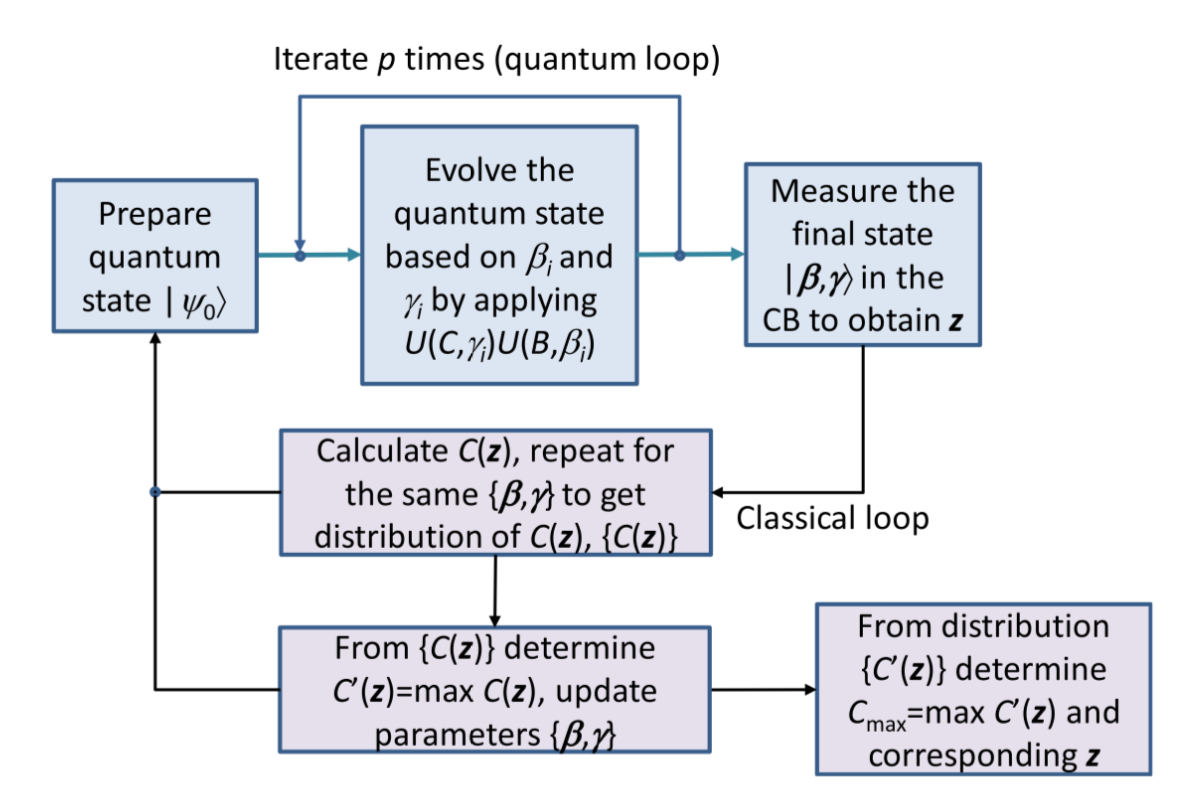
\includegraphics[width=0.8\linewidth]{qac2}
		\caption{QAOA procedure \cite{Djordjevic2021}.}
		\label{fig:qac2}
	\end{figure}
	\chapter{Application of QAOA to The Max-Cut Problem}
	\section{Problem Statement}
	We now apply QAOA to the Max-Cut problem, which is one of the most important examples in combinatorial optimization and graph theory. Given an undirected graph $G=(V,E)$, the objective is to divide the set of vertices into two disjoint subsets, say $S$ and $S'$, in such a way that the number of edges connecting vertices in opposite subsets is as large as possible. The set of edges that cross from one subset to the other is called the \emph{cut} and is denoted by $\delta$.
	
	The Max-Cut problem is interesting for two reasons. First, it has a simple graphical interpretation, which makes it a natural example for illustrating QAOA. Second, it is computationally hard in general, so it serves as a useful test case for quantum optimization algorithms. In many practical situations, one is not just interested in finding any partition, but rather the one that maximizes the number of separated edges. This makes Max-Cut a standard benchmark for both classical approximation algorithms and quantum variational methods.
	
	\section{Example of a Square Graph} \label{sqr}
	Consider a square ring with $N=4$ nodes. Since each node may be assigned to either of the two subsets, there are $2^N$ possible graph partitions in total. One convenient way to represent a partition is by using a $4$-bit string. If a particular bit belongs to the set $S$, we assign the value $1$; otherwise, we assign $0$. In this way, every binary string corresponds to one possible division of the graph into two parts.
	
	\begin{figure}[htbp]
		\centering
		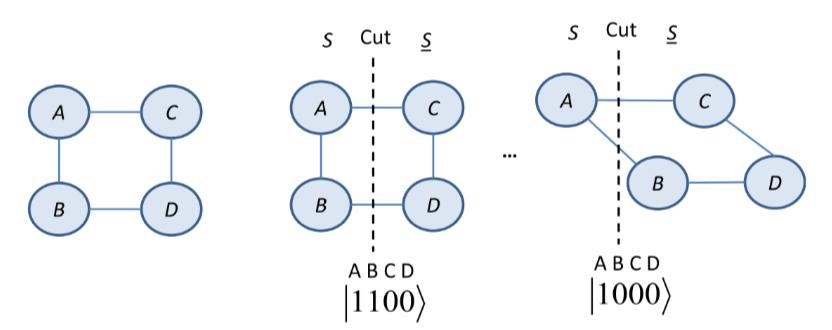
\includegraphics[width=0.8\linewidth]{screenshot001}
		\caption{Max-Cut problem \cite{Djordjevic2021}.}
		\label{fig:maxcut}
	\end{figure}
	For a given edge $\langle j,k \rangle$, define the function $C_{\langle j,k \rangle}$ to return $1$ when the two vertices $j$ and $k$ lie in different subsets, and $0$ otherwise. In other words, the function checks whether that edge is cut by the partition. The total cost function is then the sum over all such edge contributions:
	\[
	C=\sum_{\langle j,k \rangle}C_{\langle j,k \rangle}, \qquad C_{\langle j,k \rangle} = \frac{1}{2} (1-z_jz_k),
	\]
	where $z_i=+1$ if the $i$th node belongs to set $S$, and $z_i=-1$ otherwise. If the edge $\langle j,k\rangle$ is cut, then $z_jz_k=-1$, and the corresponding contribution becomes $1$. If the two vertices lie in the same subset, then $z_jz_k=+1$, and the contribution becomes $0$. Therefore, maximizing the cost function is equivalent to maximizing the number of cut edges.
	
	The objective function can again be represented as an operator:
	\[
	C\ket{z}=\sum_{\langle i,k\rangle}C_{\langle i,k\rangle}(z)\ket{z}=C(z)\ket{z}.
	\]
	This operator is diagonal in the computational basis, which makes it especially convenient for QAOA. Each basis state $\ket{z}$ represents a candidate partition, and the corresponding eigenvalue gives the number of edges cut by that partition.
	
	The corresponding unitary evolution operator for $C$ is
	\begin{equation}
		U(C,\gamma)= e^{-i\gamma C} = e^{-i\gamma \sum_{\langle j,k\rangle}C_{\langle j,k\rangle}}=\prod_{\langle j,k\rangle}U(C_{\langle j,k\rangle},\gamma),
	\end{equation}
	where
	\[
	U(C_{\langle j,k\rangle},\gamma) = e^{-i\gamma C_{\langle j,k\rangle}}=e^{-i\frac{\gamma}{2}I}e^{-i\frac{-\gamma}{2}Z_jZ_k}.
	\]
	This form shows that the cost Hamiltonian can be implemented using two-qubit interaction terms. Hence, Max-Cut provides a direct and physically meaningful example of how a graph optimization problem can be encoded into the QAOA framework.
	\chapter{Qiskit Implementation}
	In this chapter we will see the Qiskit Implementation of the MAX-CUT problem. We will deal with 2 variations of the problem stated in the section \ref{sqr}. For details about the program please refer to the Appendix \ref{app}. Here we briefly discuss the findings and the success of the simulation on a Quantum Computer Simulator called \emph{QISKIT\_AER}. 
	\section{The quantum circuit}
	As described above in section \ref{trot} and equation \refeq{qa} we will apply the horizontal and vertical approximations as unitary rotation gates. In the circuit $H$ stands for the Hadamard Gate , $R_z$ for single qubit rotation about Z-axis and the $+$ stands for a controlled Not gate \cite{nielsen}.
	
	\subsection{Case-1: n = 4 and edges = 4}
	In this case (refer to the figure \ref{fig:img2}) we have the nodes connected in a cyclic fashion $0\rightarrow1\rightarrow2\rightarrow3\rightarrow0$. The numbers on the circle identify the nodes and the respective numbers also identify with the respective qubits. For example the node 0 is denoted by $q_0$ in the circuit \ref{circ_1}.
	\begin{figure}[!htb]
		\centering
		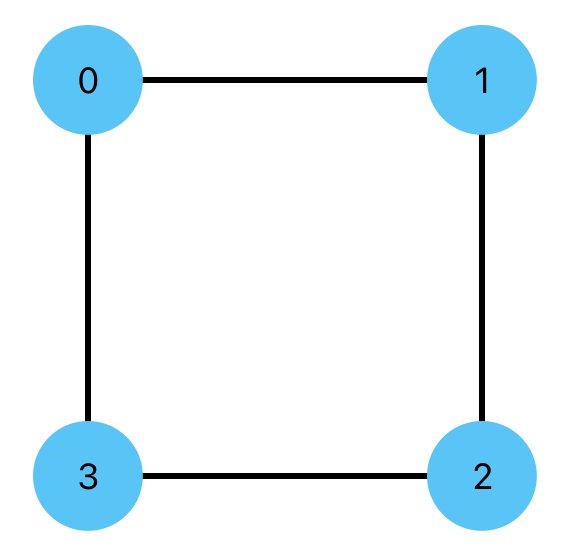
\includegraphics[width=0.25\linewidth]{img2}
		\caption{case 1 $\ket{0000}$ \cite{Quantum-Machine-Learning-QAOA}}
		\label{fig:img2}
	\end{figure}
	The circuit initializes the system by applying a Hadamard transform \cite{nielsen} of qubits . Then depending on the edges in the graph it selectively entangles two nodes, applies the rotation gate of angle $2\gamma$ (along $Z$ direction) and then reverts the entanglement. This is is then followed by a rotation gate with rotation angle of $2\beta$ (along $X$ direction). This entire process is repeated $p$ times, where $p$ is  the number of trotterization steps. If we increase p we expect to see an increase in accuracy.
	\begin{figure}[!htb]
		\centering
		\tcbox[boxsep=0em,colback=white]{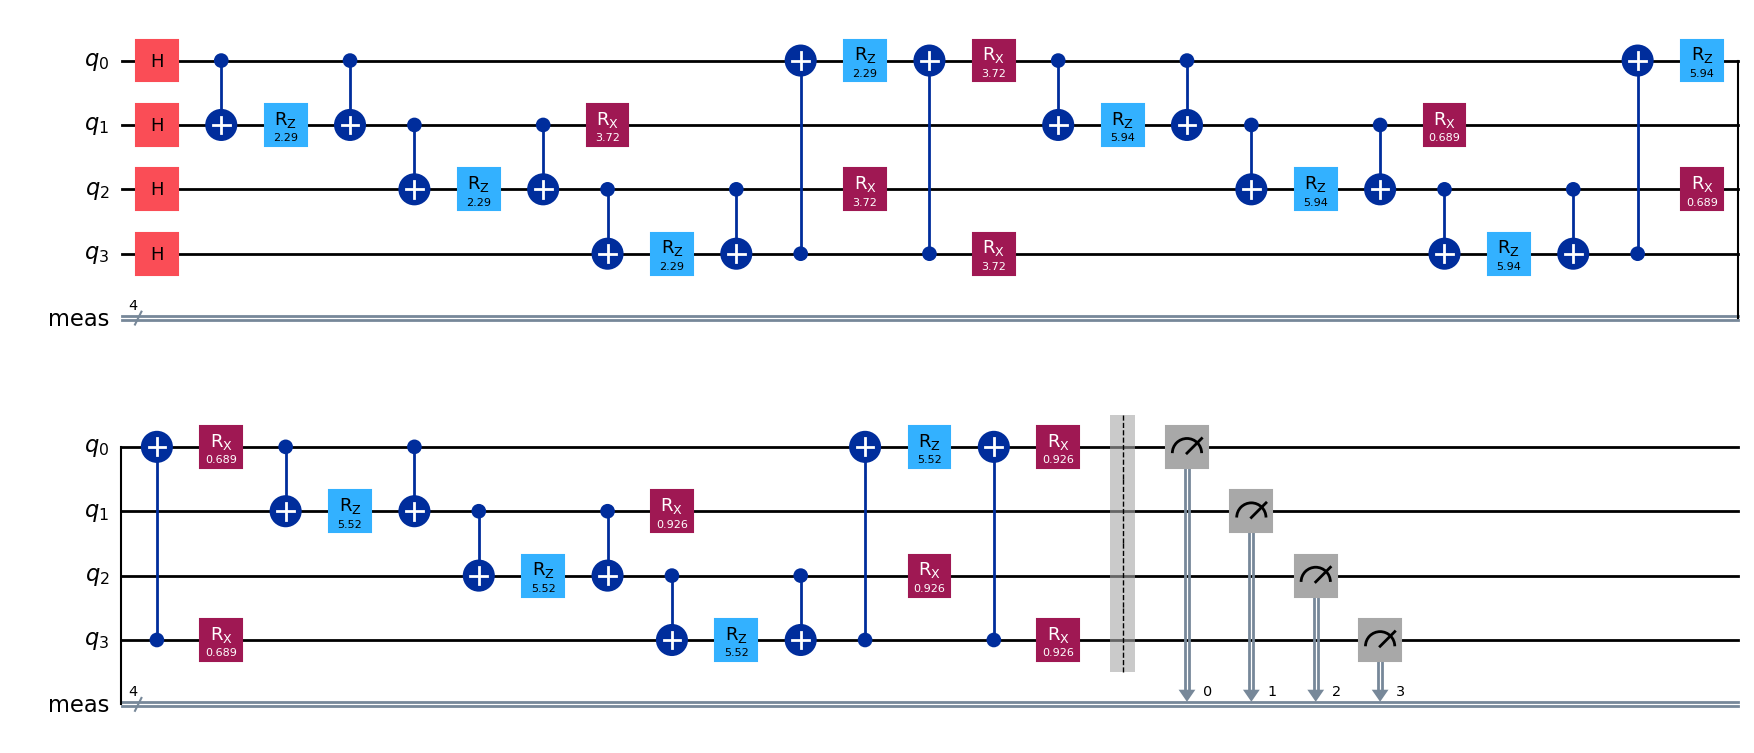
\includegraphics[width=0.9\textwidth]{circuit_1}}
		\caption{Circuit for QAOA application on a square grid with p = 3 \cite{Quantum-Machine-Learning-QAOA}.}
		\label{circ_1}
	\end{figure}
	\\
	We run this circuit with choosing initial parameters randomly and then using the\emph{ 'COBYLA}' method to optimize the cost function gradient free. Figure \ref{circ_1} shows the circuit for $p=3$ after the optimization is completed. Thus using Quantum Variational Circuit along with a Classical Optimizer we reach at the final set of parameters that yield us the solution to our MAX-CUT problem in terms of bit strings.
	\begin{figure}[!htb]
		\centering
		\tcbox[boxsep=0em,colback=white]{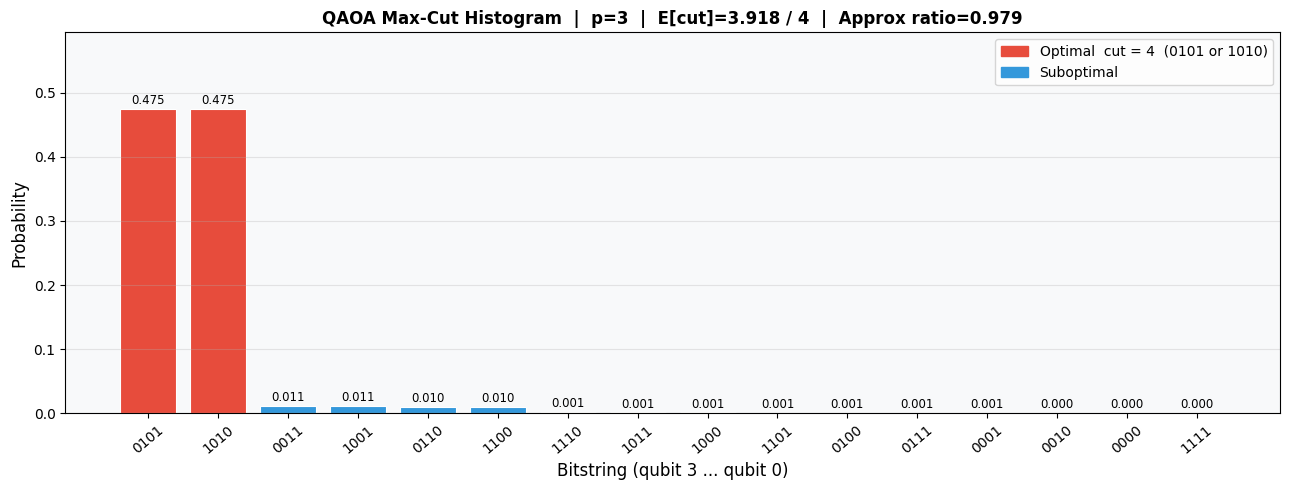
\includegraphics[width=0.98\textwidth]{plot_result_1}}
		\caption{Results of 8192 shots for case 1, p = 3. \cite{Quantum-Machine-Learning-QAOA}}
		\label{pl1}
	\end{figure}
	\\We see in the fig \ref{pl1} the bitstrings $\ket{0101}$ and $\ket{1010}$ have the maximum probability. These final states correspond to the graphs shown in fig \ref{o1}.
	\begin{figure}[!htb]
		\centering
		\begin{subfigure}{0.45\linewidth}
			\centering
		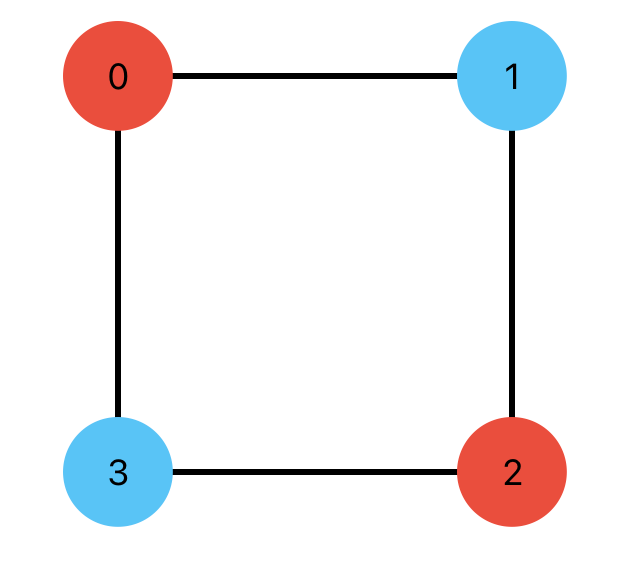
\includegraphics[width=0.5\linewidth]{o1}
		\caption{$\ket{0101}$}
	\end{subfigure}
	\begin{subfigure}{0.45\linewidth}
		\centering
		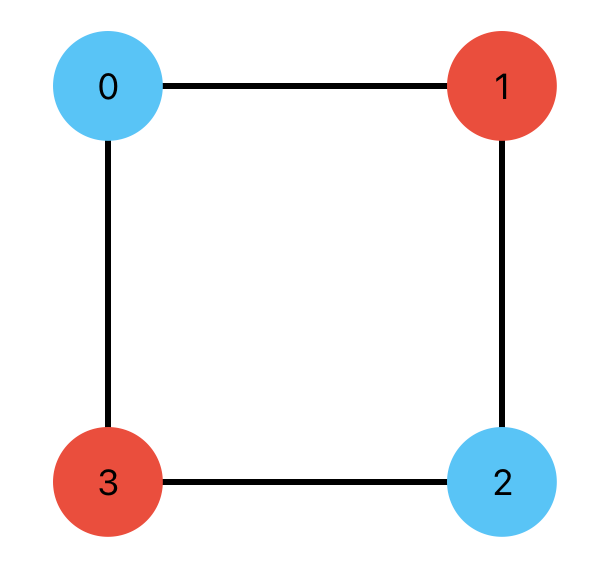
\includegraphics[width=0.5\linewidth]{o2}
		\caption{$\ket{1010}$}
	\end{subfigure}
	\caption{Solutions to case 1 of Max Cut problem}
	\label{o1}
	\end{figure}
    These two configurations have a cut value of $4$ which is the maximum that can be achieved. For detailed analysis of accuracy and $p$ value dependence refer to Appendix \ref{app}.
    \\\\\\\\\\\\
    \subsection{Case-2: n = 4 and edges = 6}
    We study a variation of the graph by adding two new edges between $0$ and $2$ \& $1$ and $3$. By addition of these new edges our circuit complexity has increased.
    \begin{figure}[!htb]
    	\centering
    	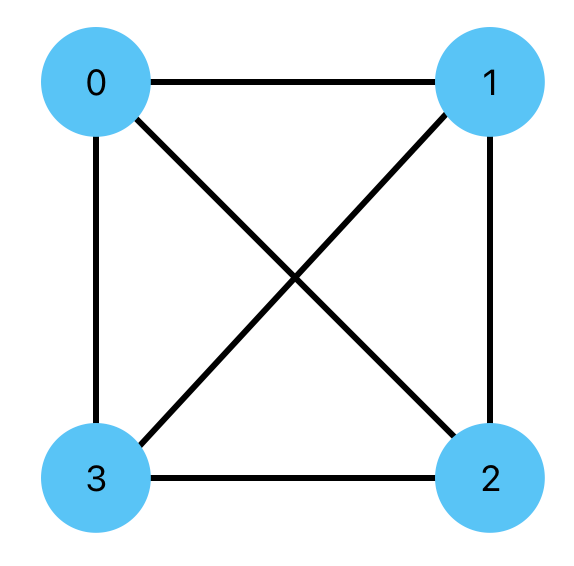
\includegraphics[width=0.27\linewidth]{graph2}
    	\caption{Case 2 $\ket{0000}$}
    	\label{fig:graph2}
    \end{figure}
    Keeping $p = 3$ we repeat the same procedure as in case 1.
    	\begin{figure}[!htb]
    	\centering
    	\tcbox[boxsep=0em,colback=white]{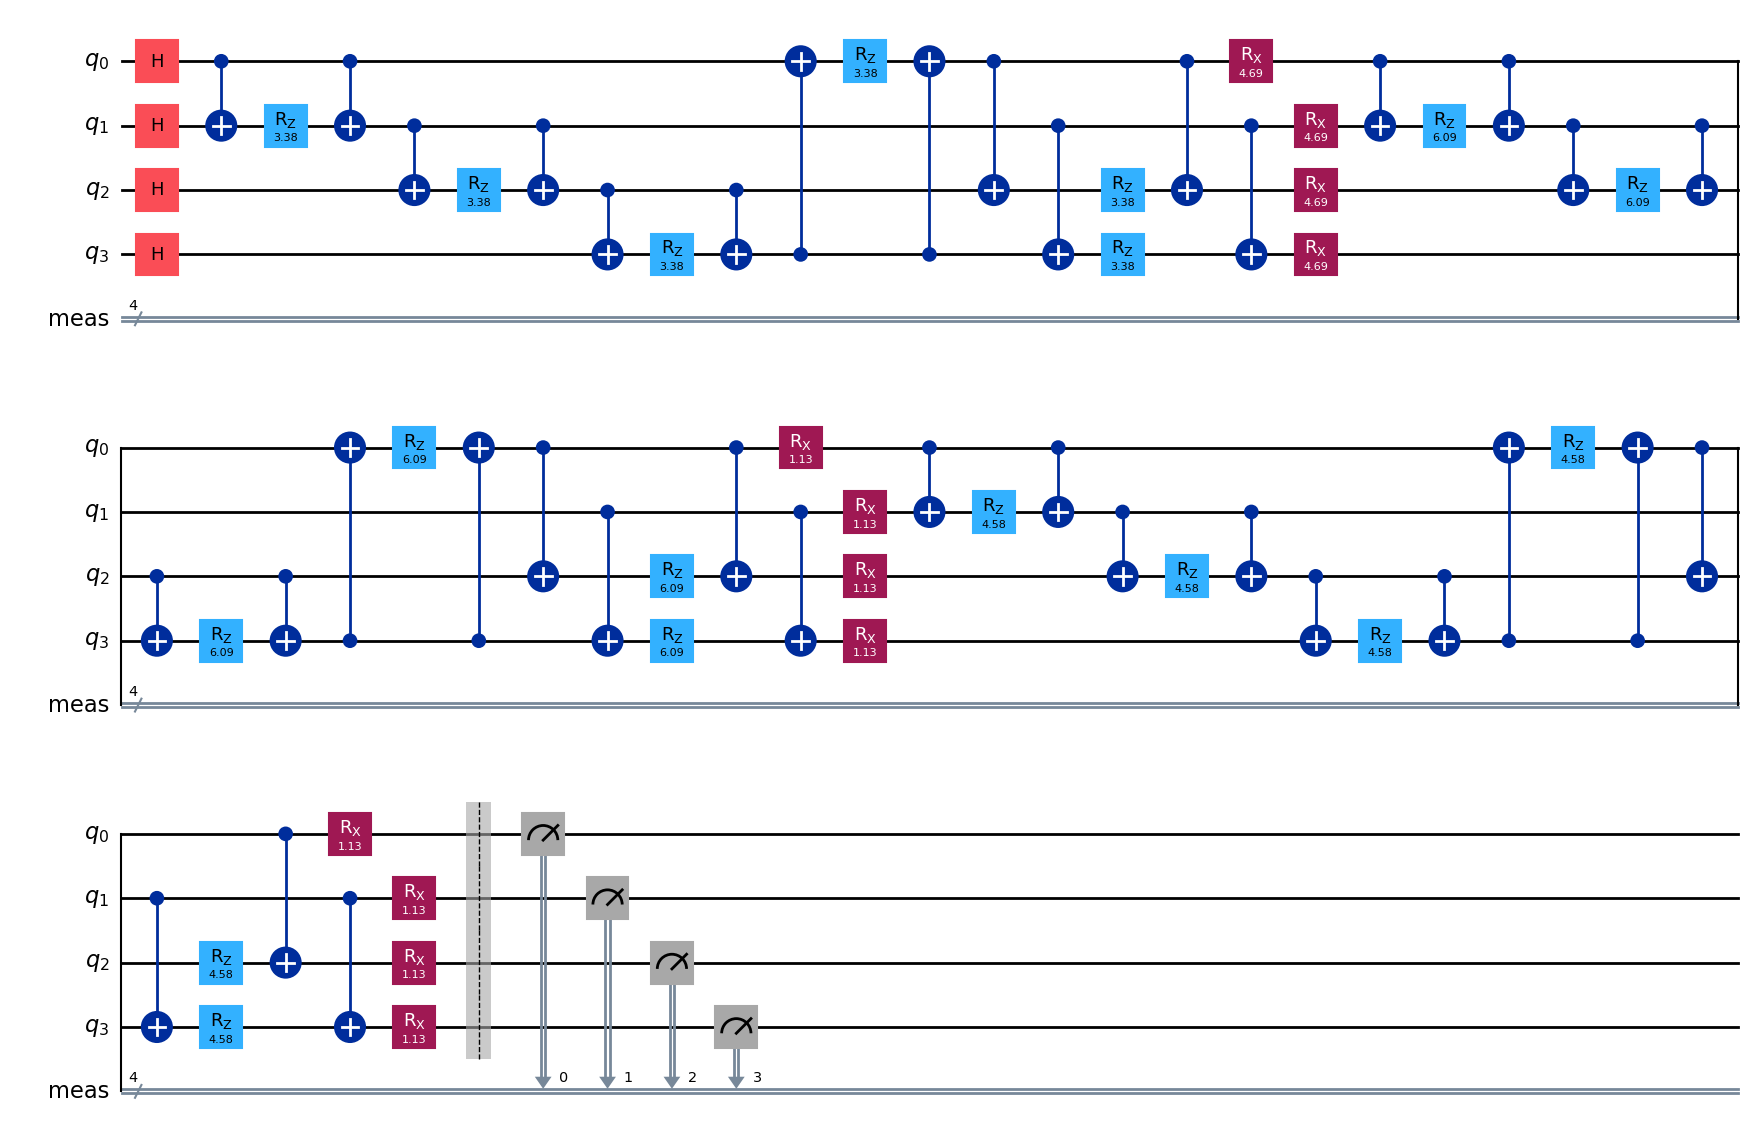
\includegraphics[width=0.7\textwidth]{circ_2}}
    	\caption{Circuit for QAOA application on a square grid with n=4 and edges = 6 and p = 3 \cite{Quantum-Machine-Learning-QAOA}.}
    	\label{circ_2}
    \end{figure}
	\\We see this time the probability distribution plot has 6 peaks in fig \ref{pl2} . \\This means there are 6 solutions to this graph.
	\begin{figure}[!htb]
		\centering
		\tcbox[boxsep=0em,colback=white]{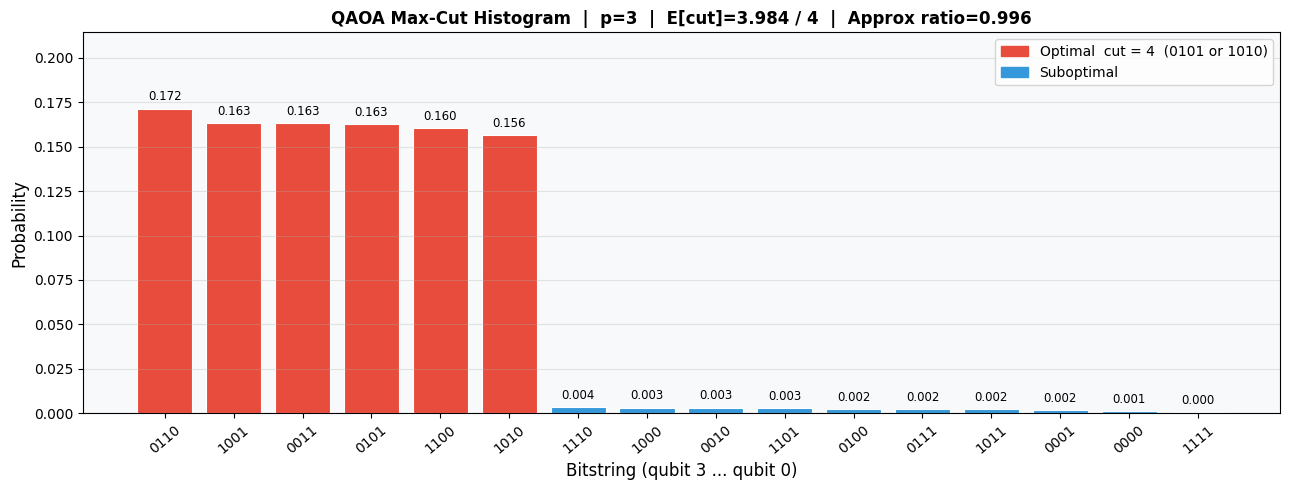
\includegraphics[width=0.98\textwidth]{plot_result_2}}
		\caption{Results of 8192 shots for case 2, p = 3. \cite{Quantum-Machine-Learning-QAOA}}
		\label{pl2}
	\end{figure}
	\\
	The solutions $\ket{0110},\ket{1001},\ket{0011},\ket{0101},\ket{1100}$, and $\ket{1010}$ are shown in Fig.~\ref{fig:case2-solutions}.
	\begin{figure}[!htb]
		\centering
		\begin{subfigure}{0.3\linewidth}
			\centering
			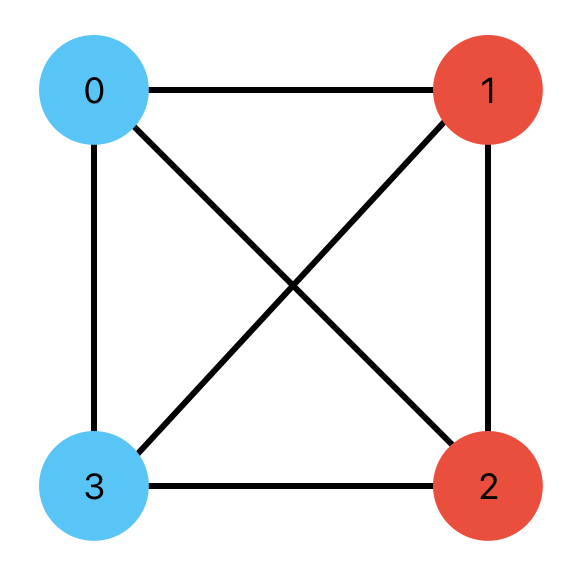
\includegraphics[width=\linewidth]{o3}
			\caption{$\ket{0110}$}
			\label{fig:o3}
		\end{subfigure}
		\hfill
		\begin{subfigure}{0.3\linewidth}
			\centering
			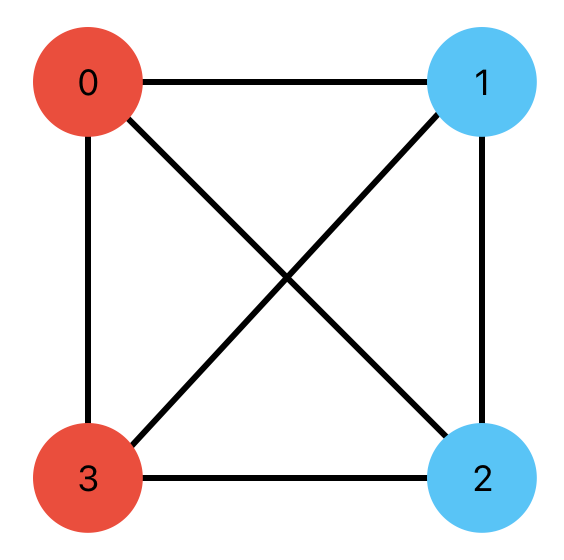
\includegraphics[width=\linewidth]{o4}
			\caption{$\ket{1001}$}
			\label{fig:o4}
		\end{subfigure}
		\hfill
		\begin{subfigure}{0.3\linewidth}
			\centering
			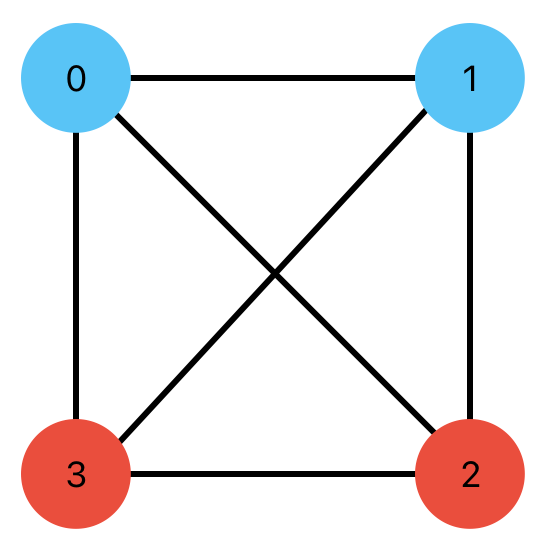
\includegraphics[width=\linewidth]{o5}
			\caption{$\ket{0011}$}
			\label{fig:o5}
		\end{subfigure}
		
		\vspace{1em}
		
		\begin{subfigure}{0.3\linewidth}
			\centering
			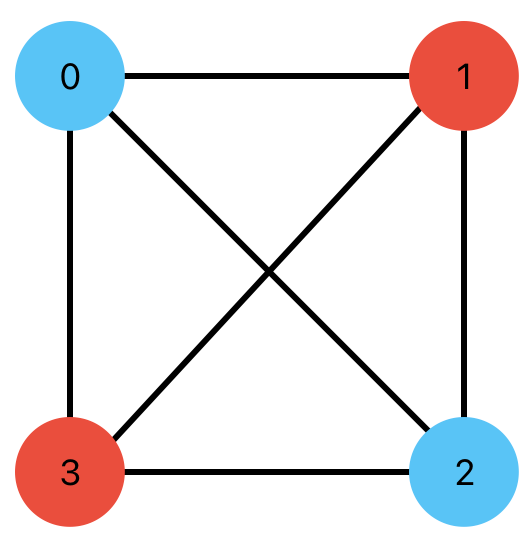
\includegraphics[width=\linewidth]{o6}
			\caption{$\ket{0101}$}
			\label{fig:o6}
		\end{subfigure}
		\hfill
		\begin{subfigure}{0.3\linewidth}
			\centering
			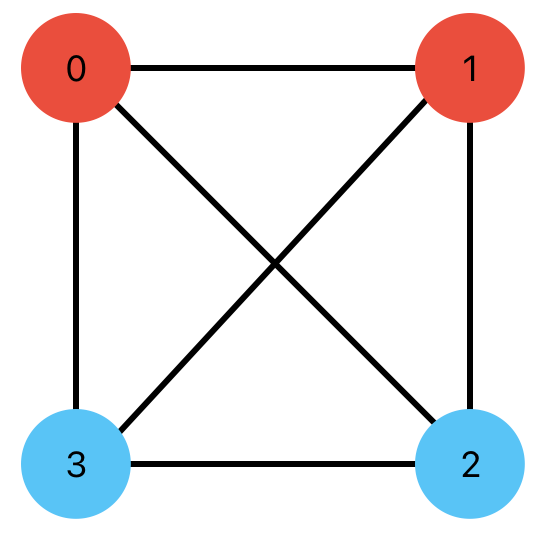
\includegraphics[width=\linewidth]{o7}
			\caption{$\ket{1100}$}
			\label{fig:o7}
		\end{subfigure}
		\hfill
		\begin{subfigure}{0.3\linewidth}
			\centering
			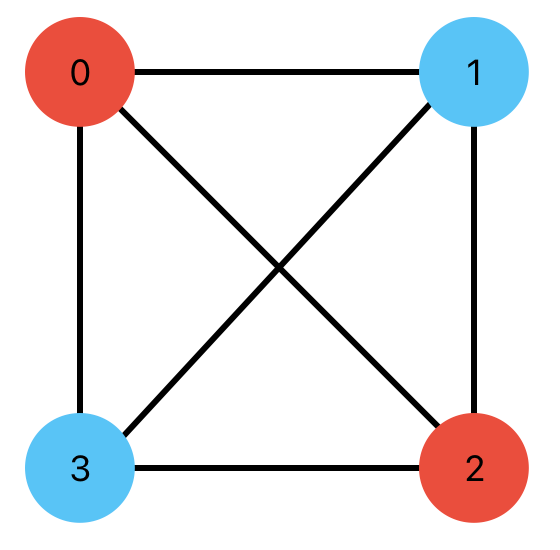
\includegraphics[width=\linewidth]{o8}
			\caption{$\ket{1010}$}
			\label{fig:o8}
		\end{subfigure}
		\caption{Solutions to case 2 of the Max-Cut problem.}
		\label{fig:case2-solutions}
		\end{figure}
	 \\All the solution correspond to a cut value of $4$.
	 \section{Results}
	 Using the Quantum Approximate Optimization Algorithm we found the maximum cut value and the configuration of a square grid for two different graphs.
	 \\\\
\emph{\textbf{	Case-1: n = 4 and edges = 4 had a max cut value of 4 and the two solutions to this were $\ket{0101}$ and $\ket{1010}$.}}
	\emph{\textbf{The Approx ratio = 0.979.}} It says the accuracy of the final evaluated expectation value of cut after classical optimization. it is defined as Expectation[cut]/Actual[cut]. As actual max cut is known to be 4 for this simple graph, we get Approx ratio to be : E[cut]/4.\\\\
\textbf{\emph{	Case-2: n = 4 and edges = 6 had a max cut value of 4 as well and there were 6 solutions: $\ket{0110},\ket{1001},\ket{0011},\ket{0101},\ket{1100}$, and $\ket{1010}$. Approx ratio = 0.996.}}
	\\\\For a graph with large n value and large number of edges, this problem becomes very difficult to solve using a classical methods and QAOA's true potential is brought into use. The study of order of operations and computation time were beyond the scope of this study and have not been included. Future prospects of this study include exploring different optimization methods during the classical processing of the data and scalability studies of the quantum processors. 
	\chapter*{Summary}
	This report presented a conceptual and mathematical introduction to the Quantum Approximate Optimization Algorithm by connecting ideas from machine learning, statistical physics, and quantum computation. The discussion began with a brief overview of machine learning and its common tasks, in order to emphasize that many practical problems can ultimately be phrased as optimization problems over structured data. Concepts such as feature vectors, similarity measures, and loss functions were introduced to build the broader context in which variational and optimization-based methods operate.
	
	The report then moved to the Ising model, which provides a natural bridge between physics and optimization. By interpreting spin configurations as binary decision variables, the search for the ground state of the Ising Hamiltonian was shown to be equivalent to solving a combinatorial optimization problem. This connection was further extended through the relation between the Ising formulation and QUBO problems, demonstrating why many discrete optimization tasks can be encoded into a form suitable for quantum algorithms.
	
	On this foundation, the report introduced the basic principles of quantum dynamics relevant to optimization, including time evolution, transverse-field Hamiltonians, adiabatic quantum computing, and quantum annealing. These ideas motivated the study of QAOA as a variational and discretized alternative to adiabatic evolution. In QAOA, the system evolves through alternating applications of a cost Hamiltonian and a mixer Hamiltonian, with the corresponding angles treated as tunable parameters optimized by a classical routine.
	The Max-Cut problem served as the main example throughout the report. It was shown how a graph partitioning problem can be translated into a cost operator that is diagonal in the computational basis, making it especially suitable for QAOA. The report described how the associated unitary operators are constructed and why the problem provides a clear illustration of how combinatorial optimization is embedded into a quantum circuit model.
	
	Finally, a Qiskit-based simulation was discussed for two four-node graph instances. The results showed that the algorithm successfully concentrates probability on the optimal bit strings corresponding to the maximum cuts, thereby illustrating the practical workflow of QAOA: parameterized circuit preparation, classical optimization, and measurement-based identification of good solutions. Overall, the report demonstrated that QAOA is not only a useful variational algorithm for near-term quantum devices, but also an important framework for understanding how physical Hamiltonians, optimization theory, and quantum circuit design come together in quantum machine learning and quantum optimization.
	
	\chapter*{Appendix}\label{app}
	The entire program and the plots are uploaded on the github repository of the username : \emph{AshisNayak-quantum} in the repository named Quantum-Machine-Learning-QAOA \cite{Quantum-Machine-Learning-QAOA}.
	\\Here we discuss the working of the python-Qiskit program used for this study.
	\bibliographystyle{unsrt}
	\bibliography{citation}
\end{document}
